%\documentclass[10pt,conference]{IEEEtran}
%\documentclass[9pt,conference]{sig-alternate}
%\documentclass[9pt,conference]{sig-alternate}
%\documentclass[10pt,print,letterpaper,nocopyrightspace]{sigplan-proc-varsize}
\documentclass[10pt,print,letterpaper]{sigplan-proc-varsize}

\usepackage{amsmath,epsfig}
\usepackage{url}
\usepackage{xspace}
\usepackage{colortbl}
\usepackage{subfigure}
\usepackage{dsfont}
\usepackage{boxedminipage}
\ifx\pdfoutput\undefined
\usepackage[hypertex]{hyperref}
\else
\usepackage[pdftex,hypertexnames=false]{hyperref}
\fi

\usepackage{amssymb}
\usepackage{wasysym}
\usepackage[left=2.54cm,top=2.54cm,right=2.54cm,bottom=2.54cm,nohead,nofoot]{geometry}



\DeclareMathOperator*{\argmax}{argmax}
%\usepackage{times}

\def\ucb{$^{\dagger}$}
\def\stanford{$^{\ddagger}$}
\def\arch{$^{\star}$}

\newcommand{\kb}{kB}
\newcommand{\rene}{Ren{\'e}\xspace}
\newcommand{\reneii}{Ren{\'e}2\xspace}
\newcommand{\wec}{WeC\xspace}
\newcommand{\mica}{Mica\xspace}
\newcommand{\micaii}{Mica2\xspace}
\newcommand{\micaz}{MicaZ\xspace}
\newcommand{\micadot}{Mica2Dot\xspace}
\newcommand{\iic}{I$^2$C\xspace}
\newcommand{\uA}{$\mu$A\xspace}
\newcommand{\dotmote}{Dot\xspace}
\newcommand{\mhz}{MHz\xspace}
\newcommand{\ghz}{GHz\xspace}
\newcommand{\kbps}{kbps\xspace}
\newcommand{\dsn}{DSN\xspace}
\newcommand{\io}{I/O\xspace}
\newcommand{\telos}{Telos\xspace}

\newcommand{\T}{\mathds{T}}
\newcommand{\XXXnote}[1]{{\bf\color{red} XXX: #1}}


\begin{document}

%\conferenceinfo{Sensys'08,} {November 5--7, 2008, Raleigh, NC, USA.}  
%\CopyrightYear{2008} 
%\crdata{978-1-60558-096-8/08/09} 

\title{StreamFS:\\A system for energy-data OLAP in buildings}
%\numberofauthors{1} 
%\author{\alignauthor Stephen Dawson-Haggerty, Jorge Ortiz, Xiaofan Jiang and David Culler\\
%\affaddr{Computer Science Division}\\
%\affaddr{University of California, Berkeley} \\ 
%\affaddr{Berkeley, California 94720} \\
%\email{\{stevedh,jortiz,xjiang,culler\}@cs.berkeley.edu}
%} 


%\subtitle{Paper \# Insert Reg Number Here}

%\title{Alternate {\ttlit ACM} SIG Proceedings Paper in LaTeX
%Format\titlenote{(Produces the permission block, and
%copyright information). For use with
%SIG-ALTERNATE.CLS. Supported by ACM.}}
%\subtitle{[Extended Abstract]
%\titlenote{A full version of this paper is available as
%\textit{Author's Guide to Preparing ACM SIG Proceedings Using
%\LaTeX$2_\epsilon$\ and BibTeX} at
%\texttt{www.acm.org/eaddress.htm}}}
%
% You need the command \numberofauthors to handle the 'placement
% and alignment' of the authors beneath the title.
%
% For aesthetic reasons, we recommend 'three authors at a time'
% i.e. three 'name/affiliation blocks' be placed beneath the title.
%
% NOTE: You are NOT restricted in how many 'rows' of
% "name/affiliations" may appear. We just ask that you restrict
% the number of 'columns' to three.
%
% Because of the available 'opening page real-estate'
% we ask you to refrain from putting more than six authors
% (two rows with three columns) beneath the article title.
% More than six makes the first-page appear very cluttered indeed.
%
% Use the \alignauthor commands to handle the names
% and affiliations for an 'aesthetic maximum' of six authors.
% Add names, affiliations, addresses for
% the seventh etc. author(s) as the argument for the
% \additionalauthors command.
% These 'additional authors' will be output/set for you
% without further effort on your part as the last section in
% the body of your article BEFORE References or any Appendices.

\numberofauthors{2} %  in this sample file, there are a *total*
% of EIGHT authors. SIX appear on the 'first-page' (for formatting
% reasons) and the remaining two appear in the \additionalauthors section.
%
\author{
% You can go ahead and credit any number of authors here,
% e.g. one 'row of three' or two rows (consisting of one row of three
% and a second row of one, two or three).
%
% The command \alignauthor (no curly braces needed) should
% precede each author name, affiliation/snail-mail address and
% e-mail address. Additionally, tag each line of
% affiliation/address with \affaddr, and tag the
% e-mail address with \email.
%
% 1st. author
\alignauthor
%Prabal Dutta\\
%       \affaddr{Computer Science Division}\\
%       \affaddr{Univ. of California, Berkeley}\\
%       \affaddr{Berkeley, CA 94720}\\
%       \email{prabal@cs.berkeley.edu}
% 2nd. author
%\alignauthor
%David Culler\\
%       \affaddr{Computer Science Division}\\
%       \affaddr{Univ. of California, Berkeley}\\
%       \affaddr{Berkeley, CA 94720}\\
%       \email{culler@cs.berkeley.edu}
% 3rd. author
%\alignauthor
%Scott Shenker\\
%       \affaddr{Computer Science Division}\\
%       \affaddr{Univ. of California, Berkeley}\\
%       \affaddr{Berkeley, CA 94720}\\
%       \email{shenker@cs.berkeley.edu}
%}
Jorge Ortiz\\
       %\affaddr{Department}\\
	\affaddr{Computer Science Division}\\
       \affaddr{University of California, Berkeley}\\
       %\affaddr{City, State Zip}\\
       \email{jortiz@cs.berkeley.edu}
}


\maketitle

%\date{14 April 2007}
%\maketitle

\begin{abstract}
Despite the growing impact of climate change and energy prices, 
per-capita energy consumption is rising. Part of the problem is visibility. We do not 
have scalable means of observing our energy consumption patterns and determining how to optimize and reduce our
consumption.
Mobile smartphones present a unique opportunity to enable an energy view on the physical world. 
They can bridge the physical world, information infrastructure, and people
through a rich set of sensors, ubiquitous connectivity, and highly personal user interface. 
With QR codes as cheap tags on items and places in the physical world, the
camera becomes a portable scanner in your pocket, in addition to its
traditional functions.  We explore this
unique triple point
and re-examine classical problems of context and consistency management in mobile
systems.  We also examine this combination as it pertains to energy management of physical
devices.  In doing so, we are re-introduced to problems of apportionment and aggregation of sensor data,
except with a continuously changing set of constituents.  We describe our solution in a technique
called \emph{dynamic aggregation} that maintains moving aggregates as the
set of data sources changes over time.  We deployed our system in a 
141,000 square-foot building, tagging 351 items over 139 room across 7 floors.

% When combined with QR codes, the on-board camera provides us with a portable scanner

% The camera,
% when combined with QR codes, gives us a portable scanner and convenient mechanism for tying these world together. 
% In this paper, we describe our system and deployment experience for a mobile phone application the provides 
% user-centric energy-view of the physical world. We describe the challenges, specifically dealing with mobility, 
% and how we address them in a set of three separate applications: an energy auditing application, a 
% device energy scanner, and a personal energy counter. We also introduce a technique called \emph{dynamic aggregation}
% which allows us to seamlessly track the constituents of aggregated energy calculations, as they move from one 
% location to another.

% Despite the recent impact of global warming and a steady increase in energy prices, 
% per-capita energy consumption is rising. Part of the problem is about visibility. We simply do not 
% have any good ways of seeing how we consume energy, and therefore, how to optimize and reduce it. 
\end{abstract}

% A category with the (minimum) three required fields
%\category{B.0}{Hardware}{General}
%\category{B.4}{Hardware}{Input/Output \& Data Communication}

%\terms{Design, Implementation, Performance, Experimentation}

%\keywords{Churn, Link, Routing, Wireless, Sensor Network, Mote}

%\newpage

\subsection{Introduction}
The United States leads the world in per-capita energy consumption.
Our electricity use has consistently increased over the last 40 years~\cite{oecd2011} and other parts of the world are rising all 
too rapidly.  With the specter of climate change and the increasing cost of energy, we must explore new
ways for individuals to gain visibility and insight into their energy consumption in order to optimize and reduce it. 
With the increasing penetration of embedded sensors in the environment and
the continued rise in smartphone adoption, we see an opportunity for smartphones to bridge the physical world
to our computational infrastructure and provide an `energy lens' on the physical world.  

We use mobile phones to construct an entity-relationship 
graph of the physical world and combine it with streaming sensor data in order to perform detailed energy-attribution.
We limit the scope of the world to a single building domain.  We have designed and implemented a real-time, mobile energy auditing
application, called the `Energy Lens', that allows us to collect information about 
things throughout the building and how they are related to each other.  For example, computer X is inside 
room Y and connected to meter Z.  Then, we use these relationships to guide our data look-up and analytical
calculations.  For example, the load curve of room Y consists of the sum of all the power traces for loads
inside room Y.  We use the mobile smartphone as the main input tool.  Our work examines \emph{three main challenges} in setting up and 
deploying a real, whole-building infrastructure to support real-time, 
fined grained energy analytics.  

The first challenge is related to tracking and mobility.
The use of mobile phones presents classical, fundamental challenges related to mobility.  Typically, mobility
refers to the phone, as the person carrying it moves from place to place.  However, in the energy-attribution
context, we are also referring to the movement of energy-consuming objects.  Tracking their relationships to spaces 
and people is as important as tracking people.  We describe how we deal with \emph{both moving people and 
moving objects} and show that these historically difficult problems can be addressed relatively easily, if the proper infrastructure is 
in place.  %We provide evidence that the approach is simple, incrementally deployable, and scalable.

The second challenge is about capturing the inter-relationship semantics and having these inform our  analytics.
We adopt the general notion of physical tags that identify objects in the world.  Our system uses \emph{QR codes} to tag things and locations 
in the physical world.  However, \emph{any tag that provides a unqiue identifier for an object could serve the same purpose}.
Once tagged, there are three types of interactions -- 
registration, linking, and scanning -- which establish important relationships.  Registration is the act of creating a virtual object 
to represent a physical one.  Linking captures the relationship between pairs of objects.  Scanning is the act of performing an item-lookup.
Each of these interactions requires a set of swiping gestures.  Linking requires two tag swipes while the other two actions
require a single tag swipe.  Internally, we maintain a \emph{entity-relationship graph (ERG)} of things, people, and locations, that gets
updated through these sets of gestures.

The third challenge is about indoor network connectivity and access.
In order to connect these components, we rely on having `ubiquitous' network connectivity.  However, in practice, network
\emph{availability} is intermittent and our system must deal with the challenges of intermittency.  We discuss how caching
and logging are used to address these challenges.  Moreover, when connectivity is re-established, we must deal with
applying updates to the ERG, as captured by the phone while disconnected.  
% Conflicts can also occur during an update.  For example, the two updates may disagree about which items are attached
% to which meters.  We implement a very simple conflict resolution scheme, described in section~\ref{sec:conflicts}.
% Finally, certain physical-state transitions are represented as a set of updates to the ERG that must be applied 
% atomically.  We implement transactions in the log-replay and transaction manager.
% Our `Energy Lens' system is deployed in a building on our campus.  We discuss
% its architecture and our design choices.  
  
% We also discuss novel strategies for tracking moving people/things and describe how we implement these in our system.  In summary, our work
% makes the following contributions:

% \begin{itemize}
% \item We design and implement a system that captures and combines physical entities, their inter-relationships, and real-time sensor data 
% 		in buildings.% using mobile phones, qr code, and a cloud-based infrastructure.
% \item We observe that certain combinations of swipes give us useful information to set the location of people and things over time.
% 		We codify this observation in our \emph{context-tracker} and use it to maintain consistency between the entity-relationship graph and the 
% 		state of the physical world.  To the best of our knowledge, this is radically different from the approaches in standard 
% 		localization techniques.  However, we argue that it can be used to \emph{enhance} their accuracy and overall performance.
% \item We implement a prefetching algorithm to obtain context-dependent information to both improve performance and
% 		enable disconnected operation.  We also design and implement a log-replay and transaction manager over our data management layer.  We describe how different conflict-resolution policies can be implemented and our rationale for the policies we chose.
% \end{itemize}

% \vspace{0.08in}

% In the next sections we go through a motivating scenario.  We then discuss some related work, followed 
% by the system architecture, evaluation, and future directions.

\section{Mapping OLAP to ERG}

\begin{itemize}
\item Introduction to OLAP.
\item Explanation of ERG in StreamFS.
\end{itemize}
Online analytical processing (OLAP) is a processing layer that provides summurization of data
from a set of underlying data repository (date warehouses).  Traditionally, OLAP is used to process
business data.  Business data summurization allows an analyst ask targetted questions about aggregates 
and trends in their data.  The data is typically multidimensional in nature and operations can be performed with
respect to those dimensions and their inter-relationship.

\subsection{Measures, Dimenions, and Levels}

\subsection{Operations: drill-down and roll-up}

\subsection{Operations: slice and dice}

\subsection{Operations: pivoting}
\section{Related work}

%\begin{itemize}
% \item dashboard
% \item andrew's lightin control work
% \item Kamin's hvac control work
% \item BEMs
% \item sMAP stuff
%\item Buildsys 2010 work~\cite{hbci}
%\item distributed consistency management: COPS
%\item mobility: tracking things with RFID~\cite{rfid_gonz2006}
%\item mobility: tracking of people, wifi indoor localization
%\item entity-relationship graphs
%\item homeOS [microsoft]
%\item HP Cooltown~\cite{cooltown}
%\end{itemize}
Our work touches on several areas from smart home research to logistics.  In the building space, there has been
some interest in building various kinds of energy-related visual and control applications.
This work focuses on the object definition, tracking, and management component of the architecture proposed by 
Hsu et al.~\cite{hbci}.  Their work stratefied the set of challenges that one could potentially face if the application 
were deployed at scale.  Our
work, in constrast, bases its design rationale on a \emph{real deployment} that is taking place at scale in a building 
on our campus.  We focus on solving fundamental systems challenges in dealing with intermittent connectivity
and conflict resolution in tracking people and things over time.  We also focus on leveraging gestures to minimize
the cost of interaction for users, while maximizing the information we can attain about the state of the world.

% Tracking people/indoor localization
An important aspect of the Energy Lens is determining when people and things have moved.  This requires some form 
of indoor localization.  There's a large body of literature in the area of indoor localization with mobile phones ranging from 
using wifi~\cite{radar}, to sonar~\cite{cricket}, to ambient noise~\cite{abs}, and a combination of sensors on the 
phone~\cite{surroundsense, darwinphone}.  Dita~\cite{dita} uses acoustic localization of mobile phones and also uses the infrastructure 
to determine gestures in free-space that are classified into pre-defined control actions.  Each of these require relatively complex 
software and/or infrastrure.  
We take a radically different, simple approach.  We use cheap, easy to re/produce tags (QR codes), place them on things in the 
environment over incrementally and use the natural \emph{swiping gesture} that users make, when interacting with the Energy Lens 
application, to track when they have moved or when the objects around them have moved.  The working principal is to attain as much 
information from their gesture to determine when something/one has moved.  We discuss our heuristics in section~\ref{sec:swipes}.

% context-aware apps
ACE~\cite{ACE} uses various sensors on the phone to infer a user's context.  The context domain consists of a set of user activities
and semantic locations.  For example, if ACE can distinguish between {\tt Running, Driving, AtHome, or InOffice}.  ACE also infers 
the one from the others, so if the user is {\tt AtHome} then they are not {\tt InOffice}.  Energy Lens uses inference to determine
when a person or thing has moved.  Certain swipe combinations give us information about whether they moved and where they moved to or
whether an item moved and where it moved to.  The main difference is that we only infer context when a user is actively swiping, rather
than a continuous approach.  Pretching is a fundamental technique used in many domains.  However, the cost of a prefetch for mobile
application outways the benefits if the prefetched data is not useful.  Informed mobile pretching~\cite{IMP} uses cost-benefit analysis 
to determine when to prefetch content for the user.  In the Energy Lens context, we prefetch data based on their location swipes.
We also rely on pretching to anticipate loss of connectivity, not just to improve preformance.

% Tracking things
Logistic systems focus on the tracking of objects as the move through distribution sites to warehouses, stores, shelves,
and purchase.  Items are tracked through bar code or RFID readers.  However, the workload is very structured and well
defined.  The authors of~\cite{rfid_gonz2006} describe this structure and leverage it to minimize storage
requirements and optimize query-processing performance.  Energy Lens uses the QR codes as the tag and the phone as an active
reader.  As objects move, users scan those items to their new location.  However, objects may belong to one or
many people, they can be metered by multiple meters a day, and their history in the system
is on-going.  In contrast, a typical logistics workload has a start (distribution site) and end point (leaving the store
after a sale).  In our workload, relationship semantics are important; we need to know whether the meter is \emph{bound-to}
rather than simple \emph{attached-to} an item.  We discuss the difference later in the paper.
% In addition to traditional logistics-style queries -- \emph{What is the average time that it took coffee-makers to move from the 
% warehouse to the shelf and finally to the checkout counter in January of 2004?} -- energy-analytics requires queries to group
% partial traces from meter data by tracking what meters the item attached to over the specified time-frame.
% The Energy Lens system collects and manages this kind of information to enable such queries.
Furthermore, we take advatange of natural gestures the user makes with the phone while scanning QR codes to extract
information about the current location of the user or things.

% Tagging items, virtual services
The key idea in the HP Cooltown~\cite{bridgingphysical,cooltown} work is to web-enable `things' in the world, grouped-by
`place', and accessed by `people' via a standardized acquisition protocol (HTTP) and format (HTML, XML).  
Cooltown creates a web presence for things in the world either directly (embedded web server) or indirectly 
(URL-lookup tag) as a web page page that display the services it provides.  Many of the core concepts in Cooltown 
also show up in Energy Lens.  The main overlap is the use of tags in the world that contain a reference to a virtual 
resource, accessible via HTTP through
a network connection.  Cooltown, however, explicitly chooses not maintain a centralized relationship
graph, it leverages the decentralized, linking structure of the web to group associated web pages together.
Furthermore, things are assumed to not move.  People are the main mobile entities.  The kind of applications
we wish to support must track where things are and their specific inter-relationships.  We imposed a richer set of 
semantics on our, centrally maintained, relationship graph and use it to provide detailed energy information.


\subsection{Namespaces}
StreamFS manages two namespaces.  The first is a flat namespaces that identifies a particular
object instance.  The second is a hiearchical namespace that identifies the current instance
of a particular object.  In this section, we discuss why we have two namespaces, how
they are managed, and how they are used by the query interface and analytical layer.

\subsubsection{Object identifier namespace}
Each new object that's created is assigned a 128-bit unique identifier:

\begin{itemize}
\item 96 high-order bits identify the object
\item 32 low-order bits identify the version of the object
\end{itemize}

In this paper we concentrate on the high-order bits used to identify the object.  Management of the low-order
bits is the subject of related, ongoing work.

\subsubsection{Hierarchical namespace}
\section{Dynamic Aggregation}
\label{sec:dynagg}
Dynamic aggregation combines the underlying entity-relationship graph with in-network aggregation.  It treats
each node in the graph as a potential point of aggregation on a particular data type.  For example,
if we need to compute aggregates of \emph{KW} data and we declare the node for a particular room as
the point of aggregation, we accept data from all children of that node that, whose units are in \emph{KW},
and add the streams together over pre-defined window size or pre-defined timeouts.

The scheme is hiearchical, so a node only accepts data from its children and only sends data to its parent.
StreamFS checks for cycles when before node insertion and prevents double-counting errors by only allowing 
aggregation-points that are roots of a tree that is a sub-graph of the entity-relationship graph.  In our deployment,
each view is a managed as an independent hierarchy.  So the hierarchy of \emph{spaces} is separate from
the \emph{inventory} hierarchy or the \emph{taxonomy} hierarchy.  This allows us to ask questions with a particular
view in mind, without conflict, and is a natural fit for our aggregation scheme.

\subsection{How it works}
Although there are different semantics applied to different node types at the application layer, StreamFS only knows
about two types of nodes: (1) default nodes and (2) stream nodes.  The main difference is that \emph{default} nodes
are not explicitly associated with data coming from a sensor and \emph{stream} nodes are.  Furthermore, default
nodes can have children, while stream nodes cannot.  In our application, meters are represented by default nodes
and each stream of data they produce is a stream node.

When an aggregation point is chosen and enabled, dynamic aggregation places a buffer at the node for the type
of data that should be aggregated.  If we want to aggregate \emph{KW} data, we specify the type and send an enable-aggregation
request to the node through an HTTP {\texttt POST} to the path for that node.  The flow of data starts at the leaves when
a stream node received data from a sensor through HTTP {\texttt POST}.  As data arrives it is immediately
forwarded upstream to the parent(s).  If a node that receives data from its children is an aggregation point it buffers
the data, otherwise it fowards it to its parent.

Ignoring the timeouts for now, lets imagine the parent is a point of aggregation and its buffer is full.  At this point
the parent separates data into bins for each source and cleans it for aggregation through interpolation.  The main
operation is to \emph{stretch} and \emph{fill} that data with linearly interpolated values.  The \emph{stretch}
operation orders all the timestamps in increasing order and for each bin (signal) interpolates the values using the
first (last) pair of data points.  If there is only a single data point, the stretch uses it as the missing value.
The \emph{fill} operation find the nearest timestamps that are less-than and greater-than the missing sampling time, 
uses their values to determine the equation of a line between them and interpolates the missing value using that equation.
Once this is done for each signal, the values are added together for each unqiue timestamp and the aggregated
signal is reported to the parent, where the operation occurs recursively to the root.
Figure~\ref{fig:aggtree} shows an illustration of its operation.  

%problem:  the buffer size has to increase exponentially up the tree, in order to not drop any values.
%solution: chuck the data into default-buffer sized pieces and parallelize the interpolation using the interpolated tasks technique


%FILL IN WITH REAL GRAPH
\begin{figure}[htb!]
\begin{center}
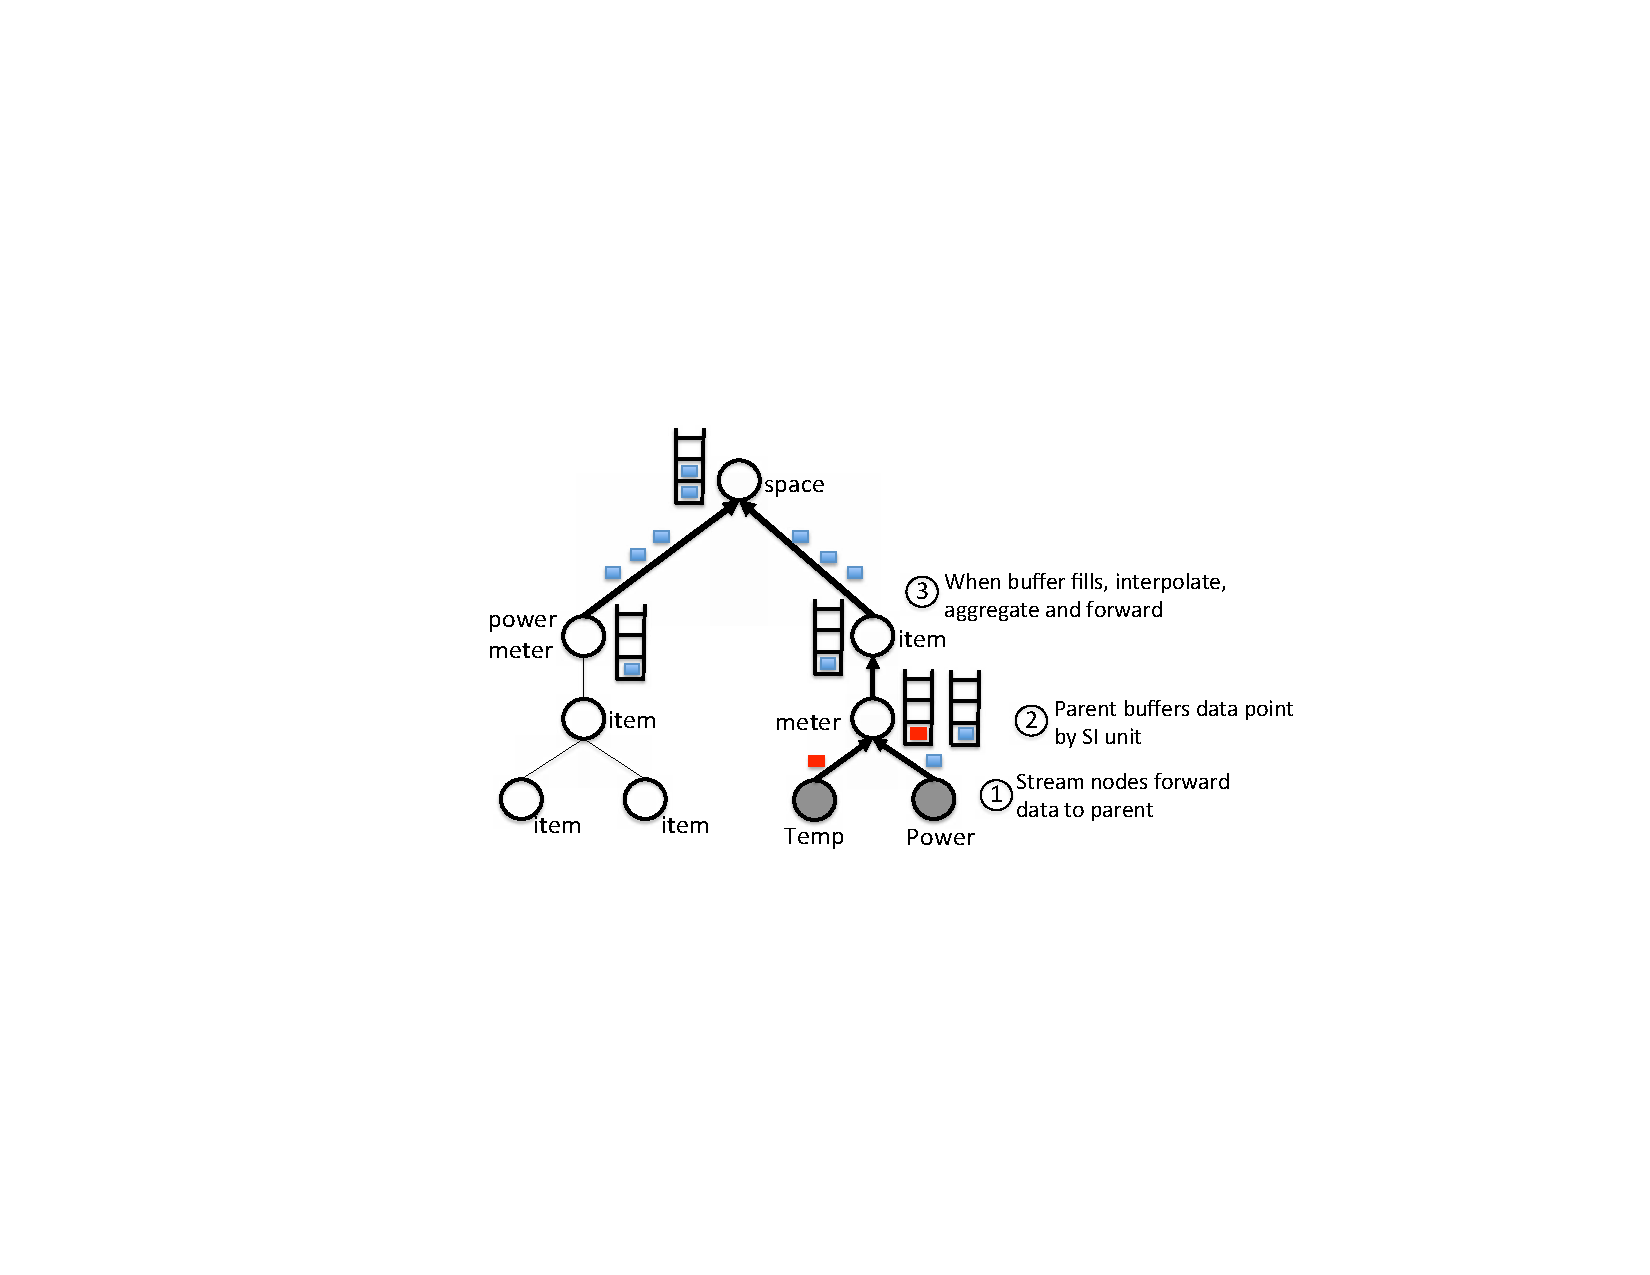
\includegraphics[scale=0.6]{figs/aggtree}
\caption{This shows an illustration of the aggregation tree used by \emph{dynamic aggregation}.  Data flows from 
the leaves to the root through user-specified aggregation points.  When the local buffer is full the streams
are separated by source, interpolated, and summed.  The aggregated signal is foward up the tree.}
\label{fig:aggtree}
\end{center}
\end{figure}

\subsubsection{Dealing with dynamics}
This approach deals with changes in the graph quite naturally.  All aggregation point deal only with local data, so
a node is only concerned about the children that give it data and the parent to send data to.  As objects in the environment
move from place to place and these changes are captured, the entity-relationship graph also changes to reflect the move.
This change in aggregation constituents is naturally accounted for in the aggregate.  If a child is removed,
it no longer forwards data to the old parent, therefore the aggregate will reflect that change.
Note, however, that changes in the entity-relationship graph are indistinguishable from energy-consuming items that have
been turned off.  For the purposes of aggregation, that is okay.

\subsubsection{Two scenarios}
We illustrate dynamic aggregation with a common usage scenario.  Imagine there are a number of people in a building,
each owning a number of plug-load applicances and a laptop.  Assume that when a person is in a room their laptop
is plugged in and when they leave the room they unplug their laptop and take it with them.  People come and go
throughout the day, changing the aggregate power consumption of the room and it happens.  In addition, some
of those people move to other rooms and plug their laptop in the new location.  As this happens, we will assume
all actions are being recorded in StreamFS.

%FILL IN WITH REAL GRAPH
\begin{figure}[htb!]
\begin{center}
\subfloat[Room 1 object and aggregate streams.]{%
            \label{fig:dynaggs1room1}
            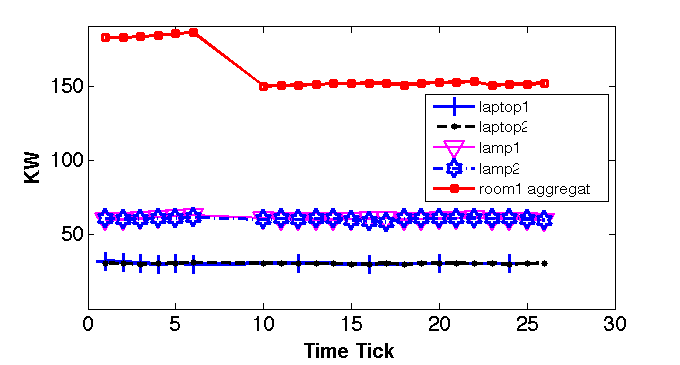
\includegraphics[scale=0.4]{figs/dynagg_scenario1_room1}
        }
\subfloat[Room 2 aggregate.]{%
            \label{fig:dynaggs1room2}
            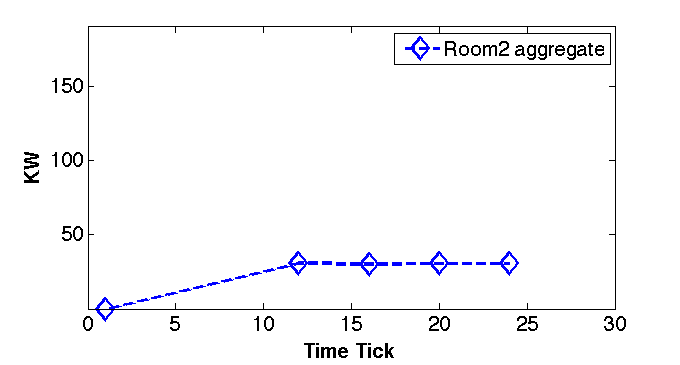
\includegraphics[scale=0.4]{figs/dynagg_scenario1_room2}
        }
\end{center}
\caption{
	The power consumes by a laptop in \emph{room 1} is shifted to \emph{room 2} a time t=7.  Notice the aggregagate drops in room 1
	while it rises in room 2.
     }%
\label{fig:multiroomagg}
\end{figure}

Figure~\ref{fig:multiroomagg} illustrate the aggregation results of that scenario.  Notice how...

% For demonstration lets have the user turn off on of their appliances when they leave as well.  This should cause that total
% room aggregate to drop, the person's personal aggregate to drop, but the other occupant's aggregate to remain
% the same.

% %FILL IN WITH REAL GRAPH
% \begin{figure}[htb!]
% \begin{center}
% 
\includegraphics[scale=0.39]{figs/blankbox}
% \caption{A room with items that belong to many users.  Person leaves with their item, aggregate falls.  Show aggregate.
% Person joins another room, aggregate in that room rises.  Show aggregate in the new room.  Compare before and after.}
% \label{fig:personaltotalagg}
% \end{center}
% \end{figure}

% Figure~\ref{fig:personaltotalagg} illustrate the results of the second sceanrio.  Note how...




\vspace{+0.5mm}
\vspace{+2mm}
\bibliographystyle{abbrv}
%\scriptsize
\bibliography{references}
%\bibliography{references}

\end{document}


